\chapter{Lecture 34 - Finite Element Method, Galerkin Method FEM in One Dimension}
\label{ch:lec34n}
\section{Objectives}
The objectives of this lecture are to:
\begin{itemize}
\item Describe a simple Galerkin FEM for solving a simple BVP.
\item Illustrate the method with a MATLAB implementation.
\item Demonstrate $hp$-refinement.
\end{itemize}
\setcounter{lstannotation}{0}

\section{Review of the Problem}

Recall the boundary value problem that we addressed in Lecture 33:
\vspace{0.25cm}

\noindent\textbf{ODE:} $ \frac{d^2 u}{dx^2} - u = -x, \ \ 0 < x < 1$

\vspace{0.25cm}

\noindent\textbf{BCs:} $ u(0) = u(1) = 0$

\vspace{0.25cm}

\noindent\textbf{Analytic solution:} $u(x) = x - \frac{\sinh{(x)}}{\sinh{(1)}}$

\vspace{0.25cm}

\noindent The strong form of the method of weighted residuals resulted in the following problem:
\begin{equation*}
\int_{0}^{1} w R \ dx = \int_{0}^{1} x(1-x) \left[-2a - ax(1-x) + x\right] \ dx = 0
\end{equation*}
that we would solve for the unknown parameter $a$.

\vspace{0.25cm}

\noindent In order to address some technical deficiencies in the method as described in its strong form, we derived the weak form:

\vspace{0.25cm}

\begin{equation*}
w \frac{d \tilde u}{dx}\Bigl|_{0}^{1}-\int_{0}^{1}\frac{dw}{dx}\frac{d\tilde{u}}{dx} \ dx - \int_{0}^{1}w \tilde{u} \ dx + \int_{0}^{1} wx \ dx = 0
\end{equation*}

\vspace{0.25cm}

\noindent In this lecture we seek to describe the Finite Element Method (FEM) as a procedure by which this weak form is solved to obtain a solution that is as accurate as we would like.

\section{Galerkin Finite Element Method}

In the finite element method, in addition to converting the strong form of the governing equation into the weak form of the minimum weighted residual statement, we will discretize the domain into a finite number of elements. For example, let us consider the one-dimensional domain divided into 3 elements, using piecewise continuous trial functions and test functions as shown in Figure \ref{fig:lec34n-discretization}.

\begin{figure}[h!]
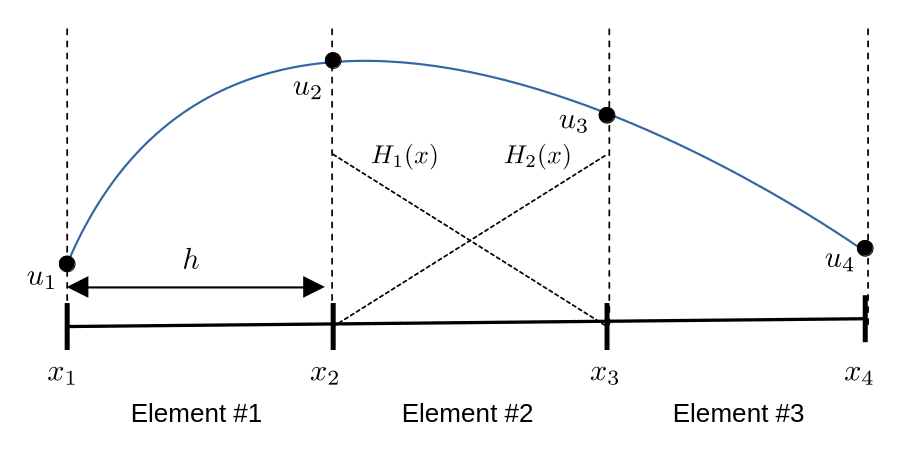
\includegraphics{lec34n-discretization.png}
\caption{Discretization of problem domain with piecewise linear elements.}
\label{fig:lec34n-discretization}
\end{figure}
\noindent Both the trial and test functions are constructed from $H_1(x)$ and $H_2(x)$ which are commonly referred to as \emph{shape functions} that are defined on each element.\marginnote[-6.0cm]{

\noindent\textbf{Note:} The shape functions, $H_1(x)$ and $H_2(x)$, are defined on each element---i.e. $H_1(x)$ and $H_2(x)$ on element \#1 are distinct from $H_1(x)$ and $H_2(x)$ on the other elements. Nonetheless, the definitions are similar for each element, namely:

\vspace{0.1cm}

\noindent $H_1(x) = \frac{x_{i+1}-x}{h_i}, \ \ H_2(x) = \frac{x - x_i}{h_i}$
where $h_i = x_{i+1}-x_i$.

\vspace{0.25cm}

\noindent $\frac{dH_1}{dx} = -\frac{1}{h_i}, \ \ \frac{dH_2}{dx} = \frac{1}{h_i}$

\vspace{0.25cm}

\noindent Notice $H_1(x_i) = 1$ and $H_1(x_{i+1})=0$ while $H_2(x_i) = 0$ and $H_2(x_{i+1}) = 1$.  This property is referred to as \emph{cardinality} of the shape functions.  Note also that $H_1(x)+H_2(x) = 1$ if $x \in [x_i,x_{i+1}]$.  Lastly note that, in principle, the element size, $h_i$, can be different for each element.  For this example, we will take the element size to be uniform.
}

\vspace{0.25cm}

\noindent\textbf{trial functions:} $u(x) = H_1(x)u_i + H_2(x)u_{i+1}$

\vspace{0.25cm}

\noindent\textbf{test functions:} $w(x) = H_1(x) + H_2(x)$

\vspace{0.25cm}

\noindent So to recap and relate to the previous discussion about the method of minimum weighted residuals: we have a piecewise linear trial and test functions; the unknown parameters are $\left\{u_1,u_2,u_3,u_4\right\}$; the test functions are ``the same'' as the trial functions insofar as that the are the same as the trial functions but without the unknown parameters.  Our goal is to solve for the unknown parameters, $\left\{u_1,u_2,u_3,u_4\right\}$, so that the weighted residual is minimized.

\newthought{Now we will} insert our newly defined trial functions and test functions into the residual:
%\begin{fullwidth}
\begin{equation*}
-\int_{0}^{1}\frac{dw}{dx}\frac{du}{dx} \ dx - \int_{0}^{1} w u \ dx + \int_{0}^{1} wx \ dx = 0 
\end{equation*}
%\end{fullwidth}

Breaking this down one component at a time, on a per-element basis:

\begin{align*}
& \frac{dw}{dx}\frac{du}{dx} = \bracketVectorstack{\frac{dH_1}{dx} \\ \frac{dH_2}{dx}} \bracketMatrixstack{\frac{dH_1}{dx} & \frac{dH_2}{dx}} \bracketVectorstack{u_i \\ u_{i+1}} = \bracketMatrixstack{\left(\frac{dH_1}{dx}\frac{dH_1}{dx}\right) & \left(\frac{dH_1}{dx}\frac{dH_2}{dx}\right) \\ \left(\frac{dH_2}{dx}\frac{dH_1}{dx}\right) & \left(\frac{dH_2}{dx}\frac{dH_2}{dx}\right)}\bracketVectorstack{u_i \\ u_{i+1}} = \left[K_1\right]\bracketVectorstack{u_i \\ u_{i+1}} \\
& wu = \bracketVectorstack{H_1 \\ H_2}\bracketMatrixstack{H_1 & H_2}\bracketVectorstack{u_i \\ u_{i+1}} = \bracketMatrixstack{\left(H_1 H_1\right) & \left(H_1 H_2\right) \\ \left(H_2 H_1\right) & \left(H_2 H_2 \right)}\bracketVectorstack{u_i \\ u_{i+1}} = \left[K_2\right]\bracketVectorstack{u_i \\ u_{i+1}} \\
& xw = \bracketMatrixstack{x_{i} & 0 \\ 0 & x_{i+1}}\bracketVectorstack{H_1 \\ H_2} = r 
\end{align*}
where, for clarity, the matrices $\left[K_1\right]$, $\left[K_2\right]$, and the vector $r$ are all functions of $x$.  Putting this all together for all 3 elements gives us:
\marginnote{
\noindent\textbf{Note:} the index $i$ corresponds to each of the 3 elements.
}
\begin{equation*}
\sum\limits_{i=1}^{3} \left[-\int_{x_i}^{x_{i+1}} \left[K_1\right]\bracketVectorstack{u_i \\ u_{i+1}} \ dx -\int_{x_i}^{x_{i+1}}\left[K_2\right]\bracketVectorstack{u_i \\ u_{i+1}} \ dx + \int_{x_i}^{x_{i+1}} r \ dx \right] = 0
\end{equation*}
This is progress but we still need to deal with the integrals.  For some problems and element types, this integration can be done analytically, but the overwhelmingly common process is to carry out the integration numerically using Gauss quadrature.

\begin{equation*}
\sum\limits_{i=1}^{3}\left[\sum\limits_{q=1}^{qp} \text{(wgt)}_q \text{(Jac)}_i \left\{ -\left[K_1(x_{q})+K_2(x_{q}) \right]\bracketVectorstack{u_i \\ u_{i+1}}  + r(x_{q}) \right\}  \right] = 0
\end{equation*}

\subsection{Assembly into a Linear System}

\begin{figure}[h!]
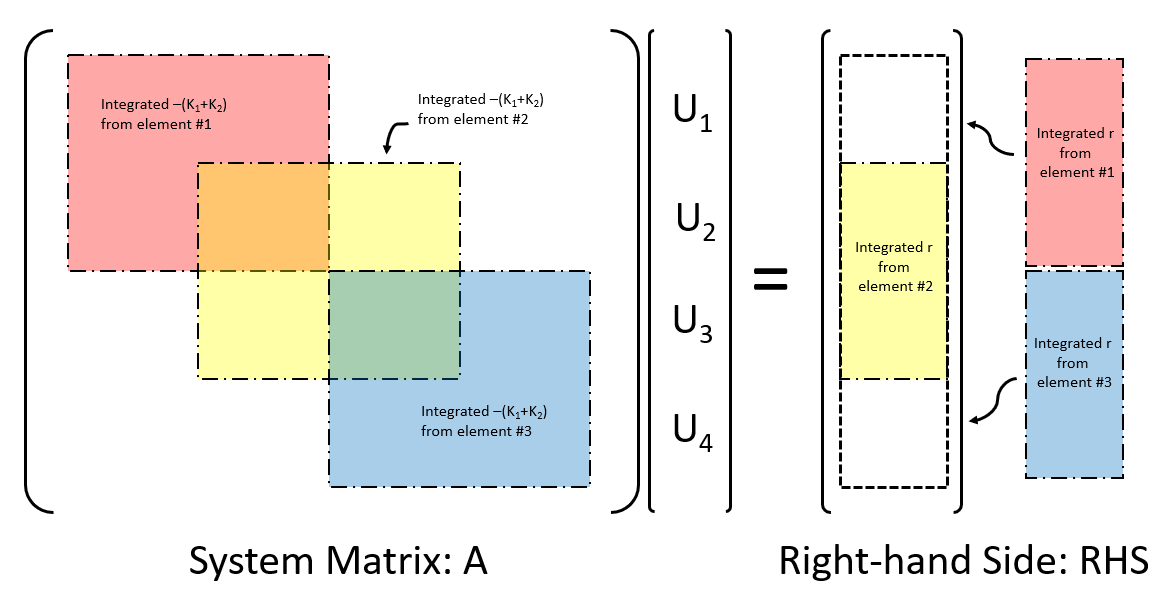
\includegraphics{lec34n-system-assembly-schematic.png}
\caption{Schematic of system assembly.}
\label{fig:lec34n-system-assembly-schematic}
\end{figure}
